\section{Introduction}

Human languages are a prime example of a culturally evolving trait: they are made up of socially learned conventions which are constantly being replicated, and exhibit great diversity across the globe~\citep{Evans2009}. Important aspects of the dynamics of language change are well-understood. Firstly, language change is \emph{sporadic}~\citep{Saussure1959,Labov2001}. Of all the conventions that make up a single language, at any given point most of them are not undergoing change, but are replicated faithfully, from basic word order patterns down to the pronounciation details of individual words. %~\citep{Pierrehumbert2002}.
Languages are transmitted robustly over many generations, a necessary requirement for their use as a tool for communication~\citep{Lewis2012}. Secondly, when a convention \emph{does} change, individuals will gradually replace an established variant with a new variant. This gradual replacement exhibits directed transitions in the form of \emph{s-shaped curves} such as the one shown in Fig.~\ref{fig:scurve}, akin to the patterns of logistic growth found in biological evolution~\citep{Bailey1973,Altmann1983,Kroch1989cr,Denison2003,Blythe2012}\footnote{While the notion of `s-shaped curves' is notoriously ill-defined, for the purposes of this paper it will suffice to use~\citeauthor{Blythe2012}'s definition as any directed trajectory that does not feature ``large fluctuations and a tendency for an upward or downward trend to reverse one or more times before an innovative variant goes extinct or wins out''~(\citeyear[p.285]{Blythe2012}).}. This similarity to the signature of adaptive selection in biology is puzzling~\citep[ch.1]{Labov2001}. Linguistic conventions are \emph{arbitrary}, which means we should not expect an inherent advantage in particular linguistic variants, such as which basic word order is used by a language, or how exactly a distinctive phonemic segment is pronounced~(as long as it maintains its contrastive function). How and why would an entire population of speakers go about replacing an existing convention with a different one ``to say the same thing''?

\begin{figure}[htb]
\centering
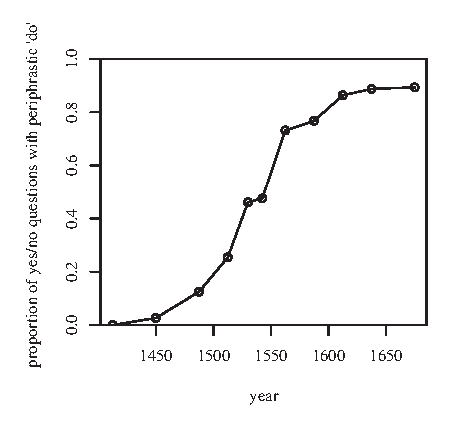
\includegraphics{scurve}
\caption[Competition between two syntactic patterns of \emph{yes/no questions}, as observed in a corpus of Middle English writing]{Competition between two syntactic patterns of \emph{yes/no questions}, as observed in a corpus of Middle English writing~\citep{Ellegard1953}. The established question syntax~(e.g.~``Went he?'') was gradually replaced by its modern variant~(e.g.~``Did he go?'') along an s-shaped trajectory.} 
\label{fig:scurve}
\end{figure}

\subsection{Language-internal accounts}

In order to explain \emph{why} languages change, many studies have attempted to pin down the causes of individual changes by systematically comparing the states of the languages prior to and after a change~\citep{Hockett1965,McMahon1994}. While many of the earliest such studies would attribute change to the gradual accumulation of performance and transmission errors alone~\citep[e.g.][]{Jespersen1922,Hockett1958}, the generativist paradigm with its focus on the language acquisition device shifted the attention to child-based language change. Studies of language change in the generative tradition have traced changes back to the re-ordering or simplification of rules~\citep{Kiparsky1968,Wang1969,Bailey1973,Lass1980,Vennemann1983}, 
assumed to be caused by children's reanalysis of linguistic parameters based on limited linguistic input~(e.g.~\citet{Ellegard1953,Lightfoot1979,Kroch1989cr,Lightfoot1991}; see \citet{Foulkes2013} for a review). % not Yang2002
Rather than characterising change as the result of imperfect transmission, a more recent strand of research regards language as a \emph{complex adaptive system} which evolves to fulfill the communicative needs of its speakers, while at the same time adapting to the constraints imposed by their learning mechanisms~\citep{Kirby1999,Steels2000,Griffiths2007,LCAS2009}.

What unites these \emph{language-internal} accounts is that they all rely on a qualitative difference between the language states prior to and after the change. This difference can be based on a variety of factors, such as the languages' expressivity, processing efficiency, or simply their stability with respect to error-prone language acquisition. Within historical and variationist linguistics such explanations of language change have long been criticised on the basis that they \emph{overpredict} change~\citep{Saussure1959,Greenberg1959,Weinreich1968,Lass1980,Ohala1989,Croft2000,Labov2001,Winter-Froemel2008}. In their seminal paper, Weinreich~et~al. succinctly summarised the issue and coined it the \emph{actuation problem}: ``Why do changes in a structural feature take place in a particular language at a given time, but not in other languages with the same feature, or in the same language at other times?''~\citep[p.102]{Weinreich1968}.

In other words, language-internal pressures by themselves do not account for the \emph{sporadicity} of language change: many non-adaptive or suboptimal structures that are claimed to have been selected against in one language will happily persist in other languages -- and when they finally do change, language-internal accounts often offer no explanation of what triggered the \emph{actuation} of the change~\citep{Saussure1959,Postal1968,Ohala1993}. While language-internal factors offer good predictions of \emph{which} changes are more likely to occur than others~\citep{Jaeger2010,Wedel2013short}, they do not explain \emph{when} or \emph{why} the stable transmission of language suddenly caves under functional pressures when it does. To account for the sporadic nature of language change, many have argued that it is not enough to rely on intra-linguistic factors alone.%~\citep{Weinreich1968,Croft2000}.

\subsection{Social accounts}

Sociolinguistic research of the past five decades has shown that innovations do not spread uniformly across a given speech community, but that the progression of change is stratified based on factors such as a speaker's age, ethnicity, or socio-economic status~\citep{Foulkes2006,Tagliamonte2012}. \emph{Social accounts} hold that social features of linguistic variants, rather than their inherent linguistic character, are responsible for driving language change~\citep{Sturtevant1947,Croft2000,Labov2001,Croft2006}. Social accounts of language change are \emph{evolutionary} in nature: they decouple the generation of \emph{variation} from the process of \emph{selection} which leads to the diffusion of variants through a speech community. The underlying mechanisms, however, are very different from biological evolution. While the generation of new variants is assumed to be driven by linguistic or functional factors, social accounts attribute the ultimate \emph{selection} of variants to extra-linguistic social factors~\citep{Ohala1989,Croft2000,Labov2001,Stevens2013}. The `division of labour' between language-internal and social pressures in this approach can simultaneously account for the arbitrary adoption of one linguistic convention from the pool of variants over another, while at the same time explaining the crosslinguistic distribution of linguistic features which reflect functional pressures.
%In general cultural evolution terminology, functional pressures generate a pool of variants that is skewed towards, 

Recent work on a mathematical model of language change suggests that only the presence of a bias which favours the replication of a newly incoming variant can reliably reproduce the s-shaped transitions observed in language change~\citep{Blythe2012}. While this mechanism, known as \emph{replicator selection}, is in principle also compatible with language-internal biases, the authors eschew this conclusion. In line with social accounts of language change they conclude instead that it is the \emph{social prestige} of a new variant that is responsible for its preferential replication. Importantly, the sociolinguistic use of the term \emph{prestige} actually refers to a \emph{content bias}: rather than preferentially copying variants used by prestigious individuals, \emph{prestige} is simply another name for a bias that, while social in origin, is actually inherent to the linguistic variant~\citep{Sturtevant1947,Labov2001}. Crucially, social accounts do not solve the underlying logical problem of how a population would agree on the selection of a new variant if there is no objective advantage to that variant. The choice of the population to attach preferential prestige to some variant is as arbitrary and requires just as much explanation as the population's increased use of one linguistic variant over another. Because variant prestige is not accounted for within the theory~\citep{Meillet1921,Labov2001} and can only be attributed post-hoc~\citep{Sankoff1988,Trudgill2004,Maegaard2013}, social accounts are typically unable to make a priori predictions about whether particular changes are likely to happen or not. If we saw competing variants as completely identical in terms of both their linguistic \emph{and} social value, % fitness
how could directed transitions come about? To address this question, it is useful to consider ideas from the wider domain of cultural evolution.

\subsection{Replicator-neutral accounts}

The evolutionary approach to language variation and change outlined above has also been adopted widely to study processes of cultural change more generally~\citep{Boyd1985,Mesoudi2011}. Interestingly, even though replicator-neutral accounts -- where individuals have no inherent preference for any of the competing variants -- have been studied extensively in the context of cultural evolution~\citep{Bentley2004,Bentley2007}, such models have received relatively little attention in the study of linguistic change~\citep[e.g.][]{Trudgill2008,Baxter2009}.

One of the attempts to build a bridge between general models of cultural evolution and the dynamics of language change is~\citet{Reali2010}. Starting from a model of pure neutral evolution by random copying -- where individuals replicate the different variants proportionally to their current frequency -- the authors add what they frame as an inferential bias for \emph{regularisation}. %, i.e.~a slight preference for individuals to adopt grammars exhibiting no variation.
They show that the trajectories produced by this `regularising' neutral model exhibit s-shaped growth, as long as only those trajectories initiated at 0\% use of a novel variant and terminating at 100\% use are considered. Crucially, however, their mathematical model captures all possible trajectories between those two points, and their result holds only for the \emph{average of all possible trajectories}. This idealised trajectory is highly unlike the `typical' transitions produced by their neutral evolution model, which are characterised by a noisy trajectory, often with many reversals. The strict symmetry of their Markov model also predicts that there should be as many completed language changes as there are actuated changes that went to the 50\% mark before being interrupted, a situation that does not seem to be the case. These considerations call into question whether neutral evolution by random copying can provide an adequate model of the dynamics of language change~\citep{Blythe2012neutral}.

While in pure neutral evolution models the likelihood of replicating a variant is assumed to be dependent on that variant's current frequency alone, another class of replicator-neutral models that has received increased attention recently considers the effects of \emph{temporal information} and \emph{memory} on the diffusion of cultural traits. % (and particularly linguistic)
\citet{Labov2001} for example suggested that the systematic incrementation of sound changes across generations could be explained by the notion of \emph{age vectors}. He hypothesises that, following an initial stage where learners acquire the average community usage of linguistic variants, adolescents advance their productions in line with the age stratification of variable usage that can be observed in the population -- in other words, it presumes that youngsters have a bias against sounding \emph{outdated}. This idea was taken up by~\citet{Mitchener2011}, who framed it in terms of \emph{prediction-driven instability}: in his mathematical model, individuals are able to observe the usage levels of a categorical sociolinguistic variable among the `older' and `younger' individuals in the population. New individuals entering the population then adopt a usage rate according to the predicted future use of the variants, by extrapolating from the usage levels of the two groups along an idealised logistic curve. While the model exhibits spontaneous transitions between the two (or more) competing language states, it produces trajectories that exhibit rapid growth from the onset of the change, unlike the gradual uptake observed in empirical data such as shown in~Fig.~\ref{fig:scurve}. %The model also relies on individuals not changing their usage frequencies once they are added to population, i.e.~
The individuals' usage rates also remain fixed after they are initally acquired, leaving open the question of whether the same mechanism could also give rise to directed changes when individuals adjust their usage rates throughout their lifetime, as has been observed in linguistic changes~\citep{Sankoff2007}.

Another general model of cultural evolution based on a similar principle is \emph{momentum-based selection}~\citep{Gureckis2009}, which we will study more closely in the remainder of the current analysis. In this model, an individual's choice between competing cultural variants is influenced by the variants' \emph{momentum}, i.e.~by \emph{changes to the variants' frequency of use} in the recent past. Individuals are assumed to be biased towards variants which have recently seen an increase in their usage rate, and conversely biased against variants that have been adopted relatively less frequently in the recent past.

\citeauthor{Gureckis2009} test their model on a dataset of the frequency of names given to children in the US over 127~years. Their prediction for the popularity of a name in a given year, which is based on the name's long-term popularity modulated by its short-term momentum, leads to a significantly better fit of the empirical data than the prediction made by pure random copying accounts which do not incorporate momentum. Importantly, their model was primarily intended to be fit to empirical data, but not meant as a generative model of individual behaviour. The authors rule this out, noting that ``if rising names are preferred, which in turn causes them to rise, then a momentum bias might quickly lead to convergence on a single token''~(p.668). They regard this as a negative property of the model, as they are interested in mechanisms that exhibit \emph{cycles} in the popularity of traits, such as found in the realm of fashion~\citep{Kroeber1919,Berger2009,Acerbi2012}. In language, on the other hand, convergence on a single convention is the rule rather than the exception, suggesting that momentum-based selection may be an appropriate model for language change.

\section{Momentum-based selection}

Our main contribution in this work is to investigate the dynamics of momentum-based selection by integrating it into an existing framework of language change, and evaluating it with respect to the characteristics of language change we identified above: the \emph{sporadic} nature of changes which, once actuated, proceed in an orderly, \emph{directed} manner. We begin by reviewing the original formulation of momentum-based selection in~\citet{Gureckis2009}. The model is built around tracking exponentially weighted moving averages~(EWMAs) of the relative frequencies of competing cultural traits over time. Given a time series of relative frequencies~$\vec{n}=\langle n_1, n_2, n_3,\dots\rangle$, the weight of each data point towards the moving average, which we denote~$\hat{n}_\alpha(t)$, decreases exponentially over time (hence the name). %The initial value is typically set to the value of the first datapoint, i.e. $\hat{n}_\alpha(0)=n_{0}$.
Given a new datum~$n_t$ received at time~$t$, the moving average is updated iteratively using
\begin{equation}
\hat{n}_\alpha(t) = \alpha\cdot n_t + (1-\alpha)\:\cdot\:\hat{n}_\alpha(t\!-\!1)\;.
\label{eq:ewma}
\end{equation}

The parameter $\alpha\in[0,1]$ is a smoothing factor that determines both the weight given to the newest data point, as well as how quickly the data points' weight decreases over time. At time~$t$, the relative weight of datum $n_{t-i}$ to the current average is $\alpha\cdot(1-\alpha)^i$. The higher~$\alpha$, the more weight is given to more recent data points. Based on this, the momentum of a variant at time $t$, $m(t)$, is determined by calculating two EWMAs $\hat{n}_\alpha(t), \hat{n}_\gamma(t)$ of the variant's attested frequencies $\langle n_1\cdots n_t\rangle$ with two distinct smoothing factors~$\gamma>\alpha$, and taking their difference,
\begin{equation}
m(t) = \hat{n}_\gamma(t) - \hat{n}_\alpha(t).
\label{eq:momentum}
\end{equation}
Because the higher $\gamma$ gives more weight to recent data points, the moving average $\hat{n}_\gamma(t)$ corresponds to the more recent popularity of a trait while $\hat{n}_\alpha(t)$ captures its long-running popularity. The momentum term $m(t)$ will consequently be positive if a variant has been more popular in the recent past compared to its long-term popularity, and negative if the variant has been adopted relatively less frequently in the recent past.

\subsection{Mathematical properties of momentum}

To understand just what is captured by the momentum term~$m(t)$, we can investigate the general dynamics of the difference between two EWMAs $\hat{n}_\alpha(t), \hat{n}_\gamma(t)$ based on their parameters $\gamma>\alpha$. %~\footnote{Readers who are not interested in the mathematical details of the model may wish to skip to the next section.}.
The strongest possible trend in changes to relative variant frequency can be achieved by initialising both EWMAs so that they indicate categorical usage of, say, the outgoing variant~(i.e.~$\hat{n}_\alpha(0)=\hat{n}_\gamma(0)=0$), and then continuously updating both EWMAs with input data suggesting that, actually, everyone is using the novel, incoming variant categorically (i.e.~$\vec{n}=\langle1,1,1,\ldots\rangle$). Even in this simple case, the dynamics of the momentum term are complex, as can be seen in Fig.~\ref{fig:ewmadifference}.

For the underlying EWMAs themselves, the higher the smoothing factor, the faster they approach the input values~(Fig.~\ref{fig:ewmadifference}a.i), and the more quickly they reflect changes in the distribution too~(Fig.~\ref{fig:ewmadifference}a.ii). The corresponding momentum terms that are derived by subtracting an EWMA with a high parameter~$\gamma$ from a more slowly changing one with a lower parameter~$\alpha$ are shown directly underneath~(Fig.~\ref{fig:ewmadifference}b). What is of interest to us are the different \emph{shapes} of these momentum curves: a parameter combination which exhibits a rapidly rising curve will cause an individual to posit a trend based on just a few suggestive input data points, while a curve that slopes off slowly means that a momentum bias will persist for a longer time after the initial detection of a trend.

Both the number of data points it takes to reach their maximum value as well as the amplitude of this highest possible momentum value depend on both smoothing factors in complex ways. The short-term memory parameter~$\gamma$ is of particular importance, as it controls the time depth at which the momentum term is most sensitive to underlying trends in the data: a high~$\gamma$ causes the momentum term to immediately reflect short-term variation in the input, while settings of~$\gamma$ closer to~$\alpha$ lead to more conservative trend estimates which smooth over the noise present in individual input data points.

The sudden change in trend after 60~data points shown in Fig.~\ref{fig:ewmadifference}b.ii illustrates this point: a momentum term based on high $\gamma=0.15$~(dotted line), while very quick to reflect sudden changes in the input, is very unstable. After receiving only five data points of the new input value $n_t=0$, the previous sustained upward trend is `forgotten', with the momentum term first quickly returning to $0$, then going negative to reflect the new, short-term downwards trend from the series of 1s back to 0s. %Momentum terms based on settings of $\gamma$ closer to $\alpha$~(e.g.~$\gamma=0.02$, dashed line) are more conservative, requiring sustained evidence of a trend over time to reach a high value.

%A value of $\gamma$ further away from $\alpha$ decreases the time until the maximally possible momentum is reached while making the overall time-course of momentum more peaky, with a higher maximum value and quicker decay back towards~$0$ following the peak.

\begin{figure}
\centering
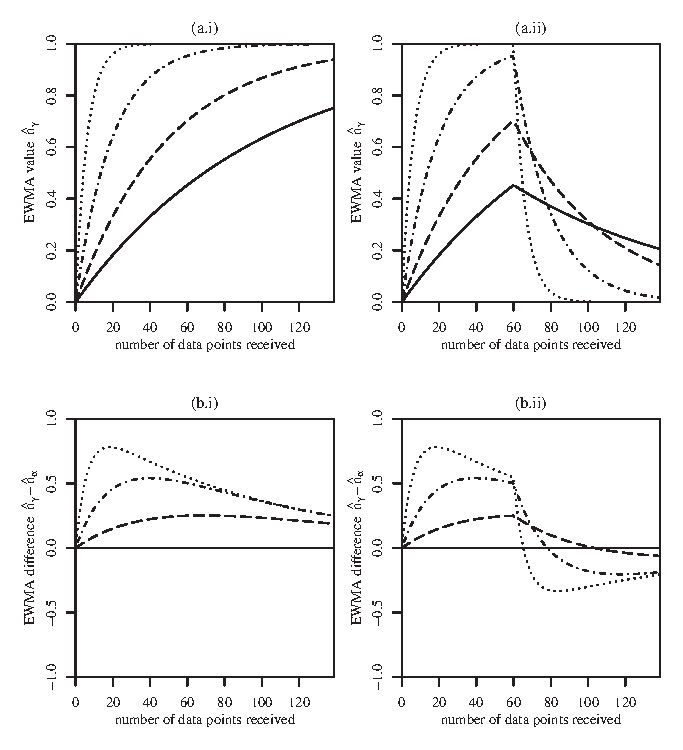
\includegraphics{ewmadifference}
\caption[Exponentially weighted moving averages~(EWMAs) of the same input data but with different smoothing factors, as well as their corresponding momentum terms]{Exponentially weighted moving averages~(EWMAs) of the same input data but with different smoothing factors, as well as their corresponding momentum terms.
% ; the slowest (solid) line shows the development of the EWMA with $\gamma=.01$, the fastest~(dotted) line $\gamma=.15$
\textit{(a.i)}~Four EWMAs with smoothing factors $\gamma=0.15, 0.05, 0.02, 0.01$~(from top to bottom) are initialised at $\hat{n}_\gamma(0)=0$ and repeatedly updated using the same constant input data series $\vec{n}=\langle1,1,1\dots\rangle$. \textit{(a.ii)}~same as~(a.i), but with the input data series $\vec{n}$ switching from all $1$s to all $0$s after 60 data points. %The EWMAs with the highest decay parameter quickly converge back towards the new input target $0$.
\textit{(b)}~Corresponding momentum terms~$m(t)=\hat{n}_\gamma(t)-\hat{n}_\alpha(t)$ derived from the trajectories above, by taking each EWMA and subtracting the value of the EWMA with the lowest smoothing factor from above~($\alpha=0.01$). Line styles correspond to those in~(a).}
\label{fig:ewmadifference}
\end{figure}

Generally, assuming an abrupt change in the input values such as above, the number of iterations that both EWMAs have to be updated with the same constant input value before the maximum possible difference between the two is reached is
\begin{equation}
t_{\rm mmax}(\alpha,\gamma)=\frac{\ln\frac{\alpha}{\gamma}}{\alpha-\gamma}\;.
\end{equation}

The maximum possible amplitude of the momentum term at that point is
\begin{equation}
m_{\rm max}(\alpha, \gamma)=e^{-\gamma t_{\rm mmax}(\alpha,\gamma)}-e^{-\alpha t_{\rm mmax}(\alpha,\gamma)}\;.
\end{equation}

Knowing the mathematical boundaries of the momentum term~$m(t)$ we can now go on to incorporate the momentum bias into a model of language change.

\subsection{The Utterance Selection Model of language change}

To investigate the dynamics of momentum-based selection as a model of individual behaviour, we implemented the momentum-based selection bias in the \emph{utterance selection model} of language change~(USM)~\citep{Baxter2006,Blythe2012}. Derived from \citeauthor{Croft2000}'s evolutionary theory of language change~(\citeyear{Croft2000}), the USM provides a well-studied multi-agent framework to study the dynamics of the competition and diffusion of \emph{discrete} linguistic replicators, be they lexical items, constructions, or different categorical variants of a speech sound\footnote{For an account of how age vectors can drive change in a continuous dimension such as vowel productions, see~\citet{Swarup2012}.}.

Two fundamental principles underlie the design of the USM: firstly, the individual agents use the competing variants \emph{proportionally}, rather than categorically. In the minimal case with only two competing variants studied here, an agent's usage rates can be fully described by a single number, call it~$x$, in the range~$[0,1]$.
While this value can be interpreted as reflecting some cognitive state of the speaker, it also has a more direct behavioural correspondent: when an agent is selected to participate in an interaction, their probability of producing the novel variant is equal to~$x$, while the probability of producing the competing variant is~$1-x$. This aspect of the USM is in line with linguistic evidence which shows that human language use is inherently variable~\citep{Kroch1994,Labov1994,Bybee2007}.

Secondly, to mimic humans' tendency to \emph{align} their linguistic behaviour with that of their interlocutors, agents continuously tune their own variable usage rate towards the production rates they observe in interactions with other agents~\citep{Jaeger2013,Nardy2013}. This aspect of the USM is in line with the finding that many aspects of linguistic behaviour do not remain fixed throughout an individual's lifetime, instead remaining malleable across the life span~\citep{Kerswill1996,Sankoff2007,LCAS2009,Bowie2013,Stanford2014handbook}. According to the formal definition of the USM~\citep{Baxter2006}, an agent's current proportion of use of a variant $x_\alpha(t)$, is simply an exponentially weighted moving average~(EWMA) of the frequencies of the incoming variant that the agent has observed in their input over time\footnote{For simplicity of notation we will henceforth omit the $\hat{}$ above the variables denoting EWMAs.}. The rate of alignment is controlled by the smoothing factor~$\alpha$ of this EWMA, which can be understood as a \emph{learning rate}. This learning rate is typically held small~(in the range of~$0.01$): there is alignment, but the individual frequency adjustments after an interaction are very small and it takes many interactions for an agent to change their preferred variant.

On top of this basic update rule, a USM agent's alignment behaviour can be altered by applying biases to their input data before it gets incorporated into the EWMA. This is where momentum-based selection comes into play.

\subsection{Momentum-based selection in the USM}

We now explain how to minimally incorporate momentum-based selection into the USM. Assuming an agent using learning rate~$\alpha$ has just engaged in its $t$-th interaction and observed another agent use the incoming variant with a relative frequency of~$y$, then their own frequency of use $x_\alpha$ is updated to be
\begin{equation}
x_\alpha(t) = \alpha\cdot f(y) + (1-\alpha)\cdot x_\alpha(t\!-\!1)\;,
\label{eq:usm}
\end{equation}
where $f(y)$ is a function from $[0,1]$ to $[0,1]$ which transforms the \emph{objective} observed frequency~$y$ of the variant into a subjective \emph{perceived frequency} which the agent then aligns to. 
Similar to \cite{Gureckis2009} we can now simply define the perceived frequency~$f(y)$ of an agent in the momentum-based USM as the objective frequency~$y$ of a variant observed in an interaction offset by that variant's momentum,
\begin{equation}
f(y) = y + b \cdot m'(t)
\label{eq:momentumusm}
\end{equation}
with the exception of
\begin{equation}
f(0)=0 \quad {\rm and} \quad f(1)=1\;.
\label{eq:momentumusmconstraint}
\end{equation}
We impose the latter since our focus lies on modelling the diffusion of existing linguistic variants, independent of how those variants were introduced into the population to begin with. It simply stops our momentum-biased selection function~$f(y)$ from introducing novel, unattested variants, a constraint that is typical of models of selection generally~\citep[see e.g.][]{Boyd1985}. The positive bias parameter~$b$ in equation~\ref{eq:momentumusm} controls the strength with which the normalised momentum term $m'(t)$ as defined below in Equation~\ref{eq:normalisedmomentum} influences the perceived frequency. Should the momentum bias cause~$f(y)$ to go below~$0$ or above~$1$, it is simply truncated at~$0$ and~$1$, respectively\footnote{The exact form of the bias function $f(x)$ matters much less than its monotonicity and the fact that $f(x)>x$ when the momentum term is positive (i.e. when the agent perceives an upward trend) and $f(x)<x$ when it is negative (indicating a downward trend).}. Crucially, because the momentum term can be positive or negative~(depending on the direction of the trend), this perceived frequency function is \emph{symmetric}, which makes it \emph{replicator-neutral}: no matter which bias strength~$b$ is used, the function does not a priori favour one of the variants over the other.

Since the effect of different strengths of this bias parameter~$b$ on the model dynamics is relevant to our analysis, we have to make sure that its settings are comparable across settings of the other parameters. This isn't as straightforward as it might seem, because the range of values that the original momentum term definition~$m(t)$ in Equation~\ref{eq:momentum} can take on depends on both smoothing factors~$\alpha$ and~$\gamma$, as could be seen in Fig.~\ref{fig:ewmadifference}. The absolute amplitude of the momentum curves is of little interest to us; on the contrary, the differences in maximum possible amplitude distort the effect of the bias parameter~$b$ which is supposed to control the strength with which momentum is applied. To counteract this, we normalise the momentum term~$m(t)$ based on the $\alpha, \gamma$ used in a given simulation condition. For any given pair of smoothing factors $\alpha, \gamma$, we can scale the momentum term to the~$[-1,1]$ range by defining the normalised momentum
\begin{equation}
m'(t)=\frac{x_\gamma(t) - x_\alpha(t)}{m_{\rm max}(\alpha, \gamma)}\;.
\label{eq:normalisedmomentum}
\end{equation}

% TODO
To calculate the momentum component in the numerator, the difference between two EWMAs, we simply re-use the agent's own usage frequency, which according to the USM definition is also an EWMA. To augment the basic USM with momentum-based selection, every agent simply has to keep track of another~$x_\gamma$ on top of the long-term estimate~$x_\alpha$ it already maintains.


\section{Results}

\subsection{Analytical approximation}

Before proceeding to a full population-based simulation we can establish the general dynamics of the model by investigating the behaviour of an individual agent set in an idealised, deterministic production-perception loop~\citep{Wedel2006}. We initialise a single agent to use the incoming variant at some low level and repeatedly update their two EWMAs $x_\alpha(t), x_\gamma(t)$ by having them align to their own proportion of use~$x_\alpha(t)$ for 100~iterations. As can be seen in Fig.~\ref{fig:feedbackloop}, nothing happens: an agent aligning to their own usage rate simply remains at that proportion and, in the absence of any changes in the input sequence, the momentum term stays~0. To test how the model reacts to fluctuations in the input we alter the agent's input by fabricating a data point which suggests that their interlocutors are actually categorically using the incoming variant~(see Fig.~\ref{fig:feedbackloop}a). When the agent aligns to this input it leads to a small punctual increase in their variant use, but the sudden change in the input data also makes the momentum term take on a positive value~(dashed grey line).
% Continuous alignment to the agent's momentum-influenced \emph{perceived} usage level~(dashed black line) leads to some further increase in the usage rate before the momentum bias tapers off towards~0.%~(
Following the fabricated data point, the agent again receives their own samples as input data. But the bias exerted by the momentum term, which makes the agent's \emph{perceived} usage rate higher than their actual usage rate, causes further increases in their use of the incoming variant. However, the lack of further perturbations causes the momentum to decay back towards~$0$, and the agent becomes stationary again at a usage level not far from their initial setting. If we introduce a second fabricated data point shortly after the first one, the model's behaviour changes dramatically: the system enters a regime where the momentum bias generated by the two fabricated data points affects the perceived frequency of the agent's input so much that it causes the momentum term to increase even further, leading to self-reinforcing runaway change~(Fig.~\ref{fig:feedbackloop}b).

\begin{figure}
\centering
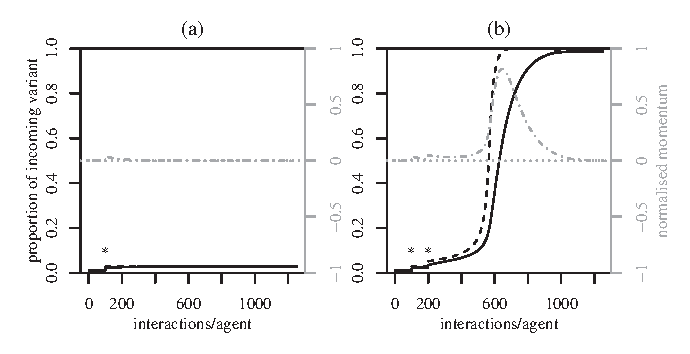
\includegraphics{feedbackloop}
\caption[Momentum-based selection dynamics of a single agent's usage rate in a deterministic production-perception loop]{Momentum-based selection dynamics of a single agent's variable usage rate in a deterministic production-perception loop, with learning rates $\alpha=0.01, \gamma=0.02$ and momentum~bias~$b=2$. At every time step the agent updates their own usage rate~(solid black line) by aligning to their own average momentum-biased production with a sample resolution of~$T=5$~(indicated by the dashed black line). This stable loop is perturbed by administering fabricated input data suggesting 100\% usage of the incoming variant at the time points marked by asterisks, demonstrating the two regimes of momentum-based selection: \textit{(a)}~stability: a single fabricated data point after 100~interactions causes a sudden increase in the agent's usage rate~(solid black line) as well as the momentum term~(dot-dashed grey line, right axis), but the feedback loop stabilises again. \textit{(b)}~directed transitions:~adding another fabricated data point after 200~interactions raises the momentum term high enough to trigger self-reinforcing runaway change, giving rise to an s-shaped transition.}
\label{fig:feedbackloop}
\end{figure}

This preliminary analysis shows that the momentum-based selection model exhibits two different regimes, accounting for both periods of stability and of directed change. Capturing the dynamics of the transition between the two regimes is however not trivial: particularly the switch from stability to a directed transition depends crucially on both the strength of the momentum bias as well as random fluctuations in the agents' input as they sample data from their interlocutors. We therefore turn to numerical simulations, where the data production and agent interactions will be driven by stochastic processes.

\subsection{Numerical simulation}

In order to get a fuller picture of the momentum-based selection dynamics we ran simulations with a total of 2,520~parameter combinations\footnote{The source code for running the simulations as well as the analytical approximation are available at \url{http://github.com/kevinstadler/momentum}}. The six parameters of the momentum-based USM are summarised below. Only one, the learning rate~$\alpha$, was held constant across all simulation runs, the other five parameters were varied at the levels given in parentheses:

\begin{itemize}
\item[-] $\alpha$: the agents' learning rate ($0.01$)
\item[-] $\gamma$: the agents' short-term memory smoothing factor~($0.015, 0.02, 0.025, 0.03, 0.35, 0.4$)
\item[-] $T$: the Binomial sample size determining the resolution at which agents can observe each other's relative usage frequencies~($2, 3, 4, 5$)
\item[-] $b$: the bias strength with which agents apply the normalised momentum to yield their \emph{perceived} frequency of usage~($0.5, 1.0, 1.5, 2.0, 2.5$)
\item[-] $N$: number of agents in the population~($2, 5, 10, 20, 30, 50, 100$)
\item[-] $x_0$: initial proportion of the incoming variant used by all agents~($0.01, 0.02, 0.03$)
\end{itemize}

Combining all these possible parameter combinations and running the 2,520~conditions for 48 trials each resulted in a total of 120,960~simulation runs. On top of the conditions listed above, we also produced simulation runs where we set the bias strength~$b=0$, which is equivalent to pure neutral evolution. 24,192~runs from this additional condition provide a baseline that the dynamics of our momentum-based selection model can be compared against. Every simulation run proceeds as follows:

Firstly, initialise $N$ agents, setting both their $x_\alpha$ and $x_\gamma$ to $x_0$. Then, carry out interactions between agents by repeating the following steps:

\begin{enumerate}
\item randomly select two agents $i, j$ from the pool of $N$ agents -- we assume that all pairs of agents have the same probability of interacting with each other.
\item let both agents produce $T$ tokens of the variable by taking a random sample $n_i, n_j$ for each agent from the Binomial distribution $B(T, x_\alpha)$, using the two agents' respective usage rates~$x_\alpha$ at the time of the interaction.
\item calculate the perceived frequencies that the agents will align to, using equation~\ref{eq:momentumusm}. For agent $i$, who will align to $j$'s productions, calculate $f(\frac{n_j}{T})$ using agent $i$'s current normalised momentum term~$m'(t)$; for agent $j$, calculate $f(\frac{n_i}{T})$ using $j$'s~$m'(t)$. %The model parameter~$b$ controls the strength with which the respective agents' momentum term~$m'(t)$ is applied.
\item update both agents' $x_\alpha$ as well as $x_\gamma$ by incorporating their perceived frequency according to equation~\ref{eq:usm}.
\end{enumerate}

The simulations were run until every individual in the population had converged to within a ten-thousandth of a percent of using only one of the two competing variants, or for a maximum of 200,000~interactions per agent\footnote{More than~$99\%$ of simulation runs had terminated before this time limit was reached.}.

\subsection{Simulation results}

For the sake of our analysis we use a simple definition of what a `transition' is. Taking a fixed threshold~(say 5\%), we can define the two extreme areas where the mean population usage level of the minority variant is below this threshold as the two regions of `near-categorical use' of either variant. A transition, then, is the period in which the mean usage levels of the population crosses from near-categorical use of one to near-categorical use of the other variant. A first striking finding when analysing the simulation results is that changes are rare: of the 120,960~simulation runs using the momentum bias, only 18,040~(around~15\%) ever exhibit a transition, while the majority of runs simply converge on categorical use of the majority variant. This result is in line with the observation that the actuation of language change is \emph{sporadic}: even when a novel variant is known to the entire population, this alone is not likely to lead to a community-wide language change.

\begin{figure}
\centering
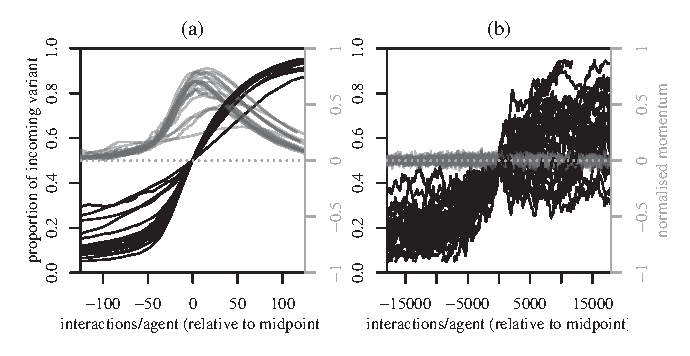
\includegraphics{alltransitions}
\caption[Successful transitions generated by simulation runs in conditions with and without the momentum-based selection bias]{Successful transitions generated by simulation runs in conditions with and without momentum-based selection. The graphs show the development of the average proportion of use of the incoming variant across the population~(black line, left axis) from the point where it crosses the 5\% mark until it reaches 95\%, alongside the average momentum term during that period~(grey line, right axis). Transitions are aligned at the point where the trajectory first crosses the $50\%$ mark of incoming variant usage. \textit{(a)}~20~trajectories randomly drawn from the 21,909 successful transitions generated by momentum-based selection with momentum bias~$b\ge1$, population sizes $N\ge5$ and various settings of $\gamma, T, x_0$. %The momentum term influences the agents' perception of the usage levels around them which, once triggered, leads to a self-reinforcing feedback loop.
\textit{(b)}~all 28 transitions generated in 17,280~simulation runs with $b=0$, equivalent to neutral evolution, with various settings of $\gamma, T, x_0$ and population sizes~$N\ge5$. %Without the influence of the momentum bias, transitions become both much rarer and slower as population size increases~
Note the different time scales. The momentum term, ineffective when~$b=0$, is shown for reference.}
\label{fig:alltransitions}
\end{figure}

When we investigate the distribution of transitions across the different parameter settings, we find that the bias strength~$b$ carves the space into two regions with distinct dynamics: while simulation runs with $b\ge1$~exhibit directed transitions at comparable time scales, the neutral evolution condition with $b=0$ as well as the weak momentum bias setting at~$b=0.5$ yield both fewer and temporally less consistent transitions, as shown in Fig.~\ref{fig:alltransitions}. The difference between those two regimes is exacerbated as population sizes become larger, making transitions in the neutral evolution conditions even rarer and slower.

Beyond this qualitative difference in successful transitions, our earlier prediction regarding the general directedness of trajectories in the neutral evolution condition are also borne out by the results: of all simulation runs where the incoming variant ever reaches the half-way mark~(i.e.~average $50\%$~usage of both variants across the population), only $55\%$ of trajectories in conditions with $b\le0.5$ actually result in the diffusion of the incoming variant. The remaining half-completed transitions are interrupted and revert back to majority usage of the established variant. In contrast, in conditions with $b\ge1.0$, $97\%$~of the trajectories that reach the half-way mark also lead to the population-wide adoption of the incoming variant.

In contrast to the low-bias conditions which exhibit the dynamics of neutral evolution, conditions with a sufficiently high momentum bias~$b$ reliably produce s-shaped transitions between the two regions of near-categorical use at irregular intervals.
%Transitions occur in both directions, which is expected given 
before eventually converging on categorical use of either of the variants. The dynamics are robust under many different parameter settings which give rise to highly similar transition dynamics~(see Fig.~\ref{fig:alltransitions}; the parameters' much greater influence on the likelihood of transitions occurring is beyond the scope of this paper). While similar transitions are also found in models driven by replicator selection, an important difference is that our model has no a priori preference for any of the variants built in. Instead of having a constant bias applied from outwith the model, the momentum term provides the opportunity for a bias to emerge dynamically from within the system, as can be seen from the temporal development of the momentum term in Figs.~\ref{fig:transitions}. Crucially, rather than relying on an external trigger, the s-shaped transitions are \emph{self-actuating}: agents constantly read weak trends into the random fluctuations in their input but these temporary individual biases will vary across the population, and more often than not cancel each other out. There is, however, always the possibility for these weak biases to overlap, which could cause a subset of agents to slowly shift their variant use in parallel. When this shift is detected by other agents they will themselves start to amplify it, leading to a self-reinforcing feedback loop. The directed transitions in a momentum-based model of language change are triggered \emph{spontaneously} and, while it is the most likely outcome, changes are not guaranteed to succeed either: even if a change is actuated, its propagation is not completely inevitable, as can be seen in interrupted changes such as the one shown in Fig.~\ref{fig:transitions}b. The dynamics of momentum-based selection provide an intriguing account of the unpredictability of the actuation of linguistic changes without the need for an external bias or trigger.

\begin{figure}
\centering
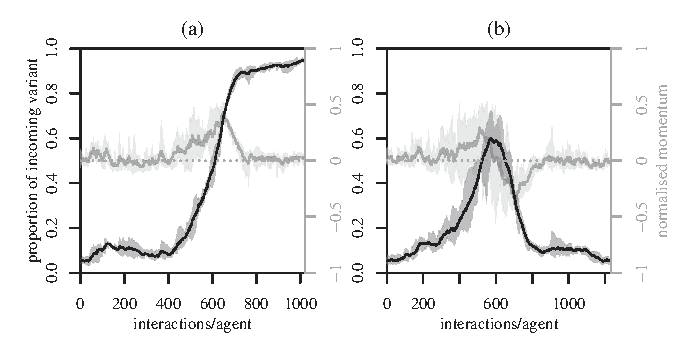
\includegraphics{transitions}
\caption[Successful and unsuccessful transitions generated by two simulation runs using identical parameter settings]{Transitions generated by two simulation runs using identical parameter settings~($N=5, b=2.0, T=2, \alpha=.01, \gamma=.04$). The graphs show the development of the average proportion of use of the incoming variant across the population~(black line, left axis) as well as the average momentum term influencing the agents' perception~(grey line, right axis). Shaded intervals indicate the range~(minimum and maximum values) attested in the population. \textit{(a)}~A successful, s-shaped transition typical of momentum-based selection: an initially noisy momentum value rises high enough to trigger self-reinforcement of the momentum bias~(at around 450~interactions) until it saturates and tails off again \textit{(b)}~Example of a rare, interrupted transition: despite the onset of a directed shift, the wide range of momentum biases across the population destabilises the feedback loop, causing the average momentum to break down and invert, returning the usage frequency of the incoming variant back towards its initial low level.}
\label{fig:transitions}
\end{figure}

The trajectories shown in Figs.~\ref{fig:transitions} are exemplary of the dynamics of momentum-based selection across the full range of parameter settings we explored. Only for settings of the momentum bias~$b$ close to~$0$ as well as for short-term smoothing factors~$\gamma$ very close to the learning rate~$\alpha$ do the momentum-based selection dynamics break down, and the model reverts to pure neutral evolution-like behaviour. In comparison to the prediction-driven model of~\cite{Mitchener2011}, the momentum-based selection model shows that it is not necessary for learners to engage in active prediction of the population's \emph{future} state along a particular trajectory. Rather, having a simple bias based on variant history is sufficient to drive orderly directed changes, and the transitions generated by our model appear to exhibit a more gradual uptake than the trajectories reported by~\citeauthor{Mitchener2011}. We also find that having a bias for \emph{regularisation} is not absolutely necessary to guarantee an orderly progression of the changes. In a population of agents who are continuously updating their usage rates, the momentum bias presented here is robust enough to drive changes to near-completion.

\section{Discussion}

We have shown that the momentum-based selection model fulfills two defining requirements of a model of language change: the spontaneous, sporadic actuation of changes, and their progression in the form of a directed, s-shaped curve. However, other accounts of language change which posit a selection bias in favour of the incoming variant also predict s-shaped trajectories, so how can we know which account best describes the empirical data? While the progression of every instance of language change will be influenced by several factors concurrently or at different times~\citep[see e.g.][]{Ghanbarnejad2014,Stanford2014handbook}, it is still interesting to investigate which (if any) of the mechanisms of language change discussed in the introduction can be identified as the main driving force behind language change. Here, we want to highlight some of the more subtle differences in the predictions made by different accounts of language change which would allow us to tease apart the momentum-based, language-internal and social accounts of language change based on cross-linguistic data.

\subsection{The two rates of linguistic change}
An interesting (and to our knowledge novel) way to evaluate competing theories of language change is to look at the predictions they make regarding the \emph{rates} of linguistic change. It is important to note that `rate' can refer to two different things in the context of language change: one interpretation of `rate' refers to the probability of a particular change occurring, such as when talking about different English past tense forms becoming regularised over time~\citep{Lieberman2007} or the rate of lexical replacement more generally~\citep{Monaghan2014}. Rather than referring to the time frame within which a specific change takes place, this really describes the \emph{likelihood of a (type of) change}, or an \emph{actuation probability}. The other use of `rate' refers to the \emph{speed} of the transition of one particular change, i.e.~it is a measure of the time span from the introduction of a new variant to its completely replacing an established one. Under the assumption that language change follows an s-shaped pattern, this second rate of change is often taken to be the growth rate parameter of the logistic function~\citep{Pintzuk2003}, and it is this `rate' that is referred to by the `Constant Rate Effect' observed in syntactic change~\citep{Kroch1989cr}.

What is interesting about these two rates of change is that different accounts of language change make implicit predictions regarding the relationship between them, in particular whether the likelihood of a change occurring is correlated with the rate at which the change proceeds once it has been actuated. Under the assumption that the same pressures that lead to the introduction of more functional or `adaptive' variants are also responsible for their preferred selection once they have been innovated, language-internal accounts would predict that changes which occur more often cross-linguistically should also be selected for more strongly in individual languages. This would translate into faster changes so that, controlling for other factors such as frequency and size of the speech community, the two rates of change should be positively correlated. % according to language-internal accounts.
This differs from the prediction made by the momentum-based account: while the probability of a new variant appearing, and consequently its random actuation from the pool of variants, is dependent on linguistic factors, these factors are not what drives the diffusion of the variant. Assuming that individuals apply similar momentum biases to all linguistic variables, a momentum-based account would therefore predict the speed of individual transitions and the changes' actuation probability to be uncorrelated.

The situation with social accounts is trickier: the fact that many different social factors have been posited to influence the selection of linguistic variants, both positively and negatively, makes it difficult to derive a general prediction regarding the speed of individual changes. What determines the probability of actuation is an equally open question: it has been proposed that the occurrence of changes might be driven by the need to create distinct social identities within a community~\citep{Labov2002,Matthews2012,Roberts2013}, implying that we should not expect actuation probabilities to be constant cross-linguistically.

While it is difficult to derive specific predictions regarding the correlation between the two rates of change from social accounts of language change, many insights into the respective roles of the different pressures could be gleaned from studying cross-linguistic datasets of changes~\citep[see also][]{Bickel2015}. The crucial issue is that the three qualitatively very different accounts discussed here might predict quantitatively similar selection pressures for particular language changes, making it impossible to distinguish the contribution of the different types of pressures on a \emph{per-change} basis. Our understanding of the issue could therefore profit immensely from investigating the empirical distribution of \emph{both} rates of change as well as their relationship based on cross-linguistic data.
%the language-internal and momentum-based accounts can be tested by investigating the correlation between the two rates of change that are attested cross-linguistically.

\subsection{Momentum-sensitivity in the individual}

While momentum-based selection successfully reproduces the macro-level s-shaped curves that are characteristic of linguistic change, this raises the question of whether the model makes valid assumptions about individuals' micro-level behaviour~\citep{Mesoudi2009}. Firstly, it is clear that both linguistic knowledge and performance are embedded in diachrony -- language users are sensitive to changes in the frequencies of variants~\citep{Jaeger2013} and well aware of diachronic connotations~\citep{Labov2001,Guy2003,Tagliamonte2012}, %,Stadler2016SS}
both types of information that could drive momentum-based selection. In the general cultural evolution literature it is well-established that frequency-dependent biases are a natural strategy for social learning tasks, since frequency can be an indicator of the \emph{social value} of a variant~\citep{Boyd1985}. Similarly, \emph{changes} in frequency can be a good indicator of the \emph{future} social value of a cultural variant~\citep{Gureckis2009}. Laboratory experiments on cultural evolution in humans have provided empirical evidence for the self-perpetuating nature of trends, where people will amplify trends even against their own personal preferences~\citep{Salganik2008,Willer2009}, suggesting that individuals might also have an incentive to use metalinguistic information about the history of linguistic variants. While there is plenty of qualitative and anecdotal evidence on speakers' explicit evaluation of language changes~(see~e.g.~\citealt{Trudgill1972,Labov2001,Guy2003,Tagliamonte2012}), quantitative research on the extent of people's explicit or implicit knowledge about the direction of ongoing changes is just starting. Experimental evidence shows that listeners employ their implicit knowledge about ongoing sound changes during speech perception~\citep{Hay2006,Drager2011}, and there is evidence of explicit knowledge both in the area of phonetic~\citep{Carrera-Sabate2014} and syntactic change~\citep{Stadler2016Evolang}. % lexical: Walker2011

%While variationist linguists customarily uncover patterns in the age distribution of linguistic variation based on collected data, quantitative forays 

\section{Conclusion}

In this paper we investigated the \emph{momentum-based selection} model and studied its evolutionary dynamics. Our analysis shows that this model, where individuals are biased towards variants which have recently seen an increase in their frequency of use, exhibits two features characteristic of language change: the spontaneous, sporadic actuation of changes, and their progression in the form of directed, s-shaped curves.

Crucially, the momentum-based selection mechanism demonstrates that the apparent selection of a particular cultural variant in a population is not sufficient evidence to conclude that there is in fact any inherent asymmetry between the variants in competition. Instead, selection biases can be an emergent property of the system, particularly in the case of social learners, where individuals possess knowledge such as about changes in the variants' frequencies of use over time.
%In our discussion we also highlighted 
Finally, we pointed to the importance of cross-linguistic data as well as the understudied capacity of individuals to detect ongoing changes, two areas which need to be investigated further to help us understand the respective roles of the different pressures involved in language change.
% us insights into the respective roles of the different accounts of language change.
%on historical language changes as an important source to  
%a number of open empirical questions related to both population-level patterns
